% ---------------------------------------------------------------- Method validation: interpretability
\subsection*{The gate is an exact, readable formula}
\paragraph{Faithfulness} For each of the \X{nGates} KAN gates fitted in the two protocols we evaluated the network and its extracted formula on the same test decision points. The largest absolute difference over all gates and points was $\X{faithMax}$ score points on the 0 to 100 scale (median over gates $\X{faithMed}$), i.e.\ floating-point agreement: the formula is the decision function. The median gate kept \X{edgesMed} active edges after pruning and its expanded formula has \X{termsMed} additive terms (largest \X{termsMax}).

\paragraph{The price of readability} Fixing the spline edges to symbolic functions is not free. On the held-out 20\% of each gate's training decision points, the mean absolute error of the stop score against the hindsight target rose from \X{maeSpline} points for the spline network to \X{maeSymbolic} points for the symbolic gate. Because the gate is used only through three wide decision bands, this loss of fit costs little in decisions (Table~\ref{tab:main}), but users who need a more precise score should keep the spline network and report its symbolic approximation instead, at the cost of exactness.

\paragraph{The deployed gate} Trained on all \nRuns{} runs (\X{depRows} decision points), the gate shipped with the controller is
\begin{equation}
s = 21.86 x_1 - 19.3 x_2 + 20.33 x_3 - 14.61 x_4 + 72.24 x_5 - 3.77 \sin{(1.49 x_3 + 6.51 )} + 34.99

\label{eq:deployed}
\end{equation}
with $x_1,\dots,x_5$ as in Eqs.~(\ref{eq:f1})--(\ref{eq:f5}), coefficients rounded to two decimals for display (the controller evaluates the unrounded expression; network and formula agree to $\X{depFaith}$ points on all recorded decision points). Fig.~\ref{fig:edges} shows each of its \X{depActiveEdges} active edge functions. An operator can read the gate's behaviour directly from Eq.~(\ref{eq:deployed}): which features push towards stopping, which towards continuing, and by how much; and for any logged decision the controller reports the score's per-feature contributions, computed from the gate itself.

\begin{figure}[t]
\centering
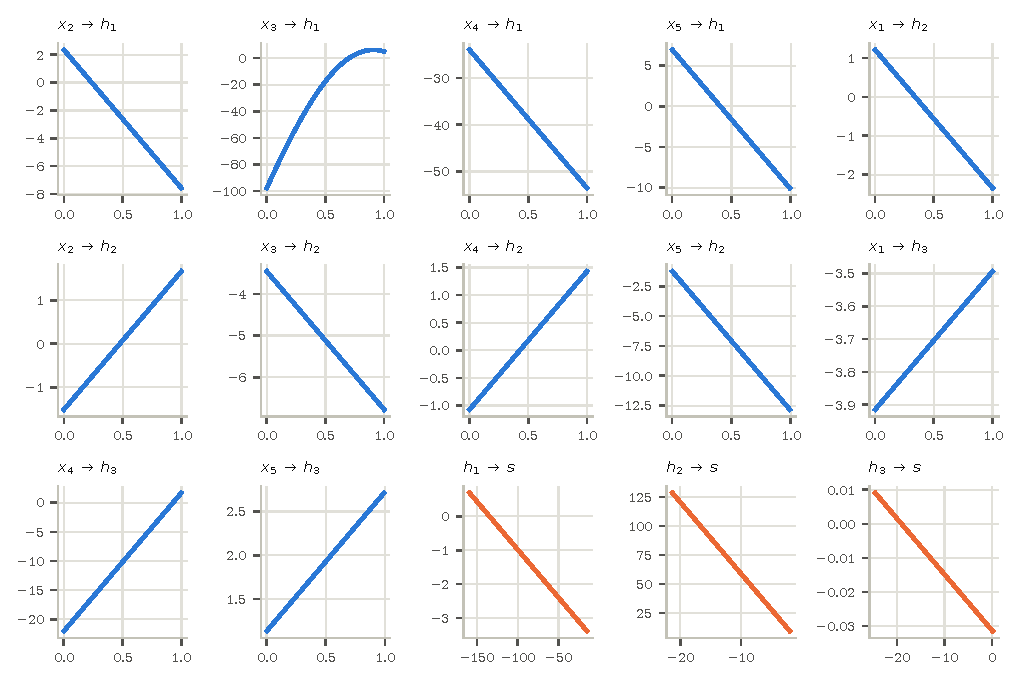
\includegraphics[width=\textwidth]{figures/edges.pdf}
\caption{Active edge functions of the deployed gate after symbolic fixing, each drawn over the range of inputs it receives on the recorded decision points. Blue: first layer (feature $x_i$ to hidden node $h_j$); orange: second layer (hidden node to stop score $s$).}
\label{fig:edges}
\end{figure}

\paragraph{Cost} Fitting a gate, including pruning and symbolic extraction, took \X{fitSeconds} s on average on a CPU, and one decision takes about \X{latKan} ms in pykan, negligible against a training epoch. Evaluating the extracted expression directly, as the static web preview of the controller does in the browser, is cheaper still.
